\subsection{Комплексные ряды Тейлора}

\begin{note}
	Формально говоря, говорить о комплексных рядах Тейлора мы не имеем права, ибо нет понятия дифференцируемости для комплекснозначных функций. Однако, мы должны прояснить тот факт, что равенство
	\[
		re^{i\phi} := r(\cos \phi + i\sin \phi)
	\]
	мы брали за определение (ну или же просто сказали, что докажем позже). Время настало.
\end{note}

\begin{definition}
	\textit{Комплексной экспонентой} называется комплекснозначная функция $e^z$:
	\[
		e^z := e^x (\cos y + i \sin y),\ z = x + iy
	\]
\end{definition}

\begin{note}
	Аналогично определяются \textit{комплексный синус и косинус}:
	\[
		\cos z := \frac{e^{iz} + e^{-iz}}{2}
	\]
	\[
		\sin z := \frac{e^{iz} - e^{-iz}}{2i}
	\]
\end{note}

\begin{theorem}
	Для $\forall z \in \Cm$ верно, что
	\[
		e^z = \row{n = 0}{\frac{z^n}{n!}};\ \cos z = \row{n = 0}{(-1)^n \frac{z^{2n}}{(2n)!}};\ \sin z = \row{n = 0}{(-1)^n \frac{z^{2n + 1}}{(2n + 1)!}}
	\]
\end{theorem}

\begin{proof}
	Воспользуемся рядами вещественных функций:
	\[
		e^x = \row{n = 0}{\frac{x^n}{n!}};\ \cos y = \row{n = 0}{(-1)^n \frac{y^{2n}}{(2n)!}};\ \sin y = \row{n = 0}{(-1)^n \frac{y^{2n + 1}}{(2n + 1)!}}
	\]
	Распишем выражение $\cos y + i\sin y$ (переставляем мы члены, благодаря абсолютной сходимости):
	\[
		\cos y + i\sin y = \row{n = 0}{\frac{(iy)^{2n}}{(2n)!}} + \row{n = 0}{\frac{(iy)^{2n + 1}}{(2n + 1)!}} = \row{n = 0}{\frac{(iy)^n}{n!}}
	\]
	Отсюда получаем $e^z$ через произведение по Коши:
	\begin{multline*}
		e^z = e^x(\cos y + i\sin y) = \row{n = 0}{\suml_{k = 0}^n \frac{x^k}{k!} \cdot \frac{(iy)^{n - k}}{(n - k)!}} = \row{n = 0}{\frac{1}{n!}\suml_{k = 0}^n C_n^k x^k (iy)^{n - k}} =
		\\
		\row{n = 0}{\frac{(x + iy)^n}{n!}} = \row{n = 0}{\frac{z^n}{n!}}
	\end{multline*}
	Для синуса и косинуса ряды уже по определению через доказанную экспоненту.
\end{proof}

\begin{proposition}
	Для комплексной экспоненты верны следующие свойства:
	\begin{enumerate}
		\item \(e^{z_1 + z_2} = e^{z_1} \cdot e^{z_2}\)
		
		\item \(e^{-z} = 1 / e^z\)
	\end{enumerate}
\end{proposition}

\begin{proof}
	Положим $\forall z_1 = x_1 + iy_1,\ z_2 = x_2 + iy_2$. Тогда
	\begin{itemize}
		\item \(e^{z_1 + z_2} = e^{x_1 + x_2} (\cos(y_1 + y_2) + i\sin(y_1 + y_2)) = \big(e^{x_1}(\cos y_1 + i\sin y_1)e^{x_2}(\cos y_2 + i\sin y_2)\big) = e^{z_1} \cdot e^{z_2}\)
		
		\item \(e^{-z} = e^{-x}(\cos(-y) + i\sin(-y)) = \frac{1}{e^x} \cdot \frac{1}{\cos(y) + i\sin(y)} = \frac{1}{e^z}\)
	\end{itemize}
\end{proof}

\section{Меры Жордана и Лебега}

\begin{note}
	Забегая вперёд, мера Жордана, вообще говоря, мерой не является. В иностранных статьях она называется не <<Jordan measure>>, а <<Jordan content>>.
\end{note}

\begin{anote}
	Я бы переводил <<Jordan content>> как \textit{содержание Жордана}.
\end{anote}

\subsection{Объём на кольце элементарных множеств}

\begin{note}
	Через $\trbr{a; b}$ будем обозначать \textit{конечный промежуток}, то есть что-то из $[a; b], [a; b), (a; b], (a; b)$.
\end{note}

\begin{definition}
	\textit{Брусом в $\R^n$} назовём множество $P$:
	\[
		P = \prodl_{k = 1}^n \trbr{a_k; b_k} = \trbr{a_1; b_1} \times \ldots \times \trbr{a_n; b_n}
	\]
\end{definition}

\begin{definition}
	\textit{Объёмом бруса $P$} назовём число $|P|$:
	\[
		|P| = \prodl_{k = 1}^n (b_k - a_k)
	\]
\end{definition}

\begin{anote}
	В иностранной литературе (в частности, в пособии по мерам от Теренса Тао) встречается не объём, а \textit{элементарная мера}.
\end{anote}

\begin{proposition}~
	\begin{enumerate}
		\item Если $P \subset Q$ - брусья, то $|P| \le |Q|$
		
		\item Если брус $P = \bscupl_{i = 1}^m P_i$, то $|P| = \suml_{n = 1}^m |P_i|$ \textit{(Конечная аддитивность объёма на множестве брусьев)}
	\end{enumerate}
\end{proposition}

\begin{proof}
	Тривиально.
\end{proof}

\begin{definition}
	$M$ называется \textit{элементарным множеством}, если оно представимо объединением конечного числа брусьев.
\end{definition}

\begin{note}
	В определении выше можно говорить о дизъюнктном объединении. Доказывается рукамаханием, с тем, что два пересекающихся бруса есть объединение нескольких непересекающихся, а дальше индукция по количеству брусьев. Далее мы будем нередко опираться именно на это определение.
\end{note}

\begin{definition}
	\textit{Объёмом элементарного множества} $M = \bigsqcup\limits_{i = 1}^m P_i$ называется число $|M|$:
	\[
		|M| = \suml_{i = 1}^m |P_i|
	\]
	Разбиений на $P_i$ вообще говоря много, поэтому то что это определение корректно и суммы у всех разбиений совпадают, нам ещё предстоит доказать.
\end{definition}

\begin{theorem}
	(Определение объёма элементарного множества корректно, т.е. не зависит от разбиения)
\end{theorem}

\begin{proof}
	Пусть \(M = \bscupl_{i = 1}^m P_i = \bscupl_{j = 1}^k Q_j\). Тогда, существует третье разбиение $M$, записываемое в следующем виде:
	\[
	M = \bscupl_{i = 1}^m \bscupl_{j = 1}^k P_i \cap Q_j
	\]
	В силу конечной аддитивности объёма на брусьях (здесь, например, мы представили $P_i$ как дизъюнктное объединение кусочков-пересечений с $Q_j$-ми), имеет место следующее равенство:
	\[
	|M| = \sum_{i = 1}^m \sum_{j = 1}^k |P_i \cap Q_j| = \sum_{i = 1}^m |P_i| = \sum_{j = 1}^k |Q_j|
	\]
	Здесь Лукашов принимает очевидным, что если мы разбили брус на конечное число брусьев, то сумма объёмов кусочков будет равна целому. (И просто двумя способами собирает из кусочков, либо первое разбиение $M$, либо второе).
\end{proof}

\begin{anote}
	Автор не считает утверждение выше таким уж очевидным но в то же время понимает ключевым в начальной теории. И потому изложит здесь описание его доказательства. Итак, ещё раз хотим доказать до боли очевидное утверждение, если брус разбит на не пересекающиеся брусья, то его объём равен сумме их объёмов. \\
	Для начала заметим что это утверждение верно, если брус разбит решёткой $n-1$-мерных плоскостей. (См. картинку, как трёхмерный пример того, что имеется в виду.)
	\\
	\centering
	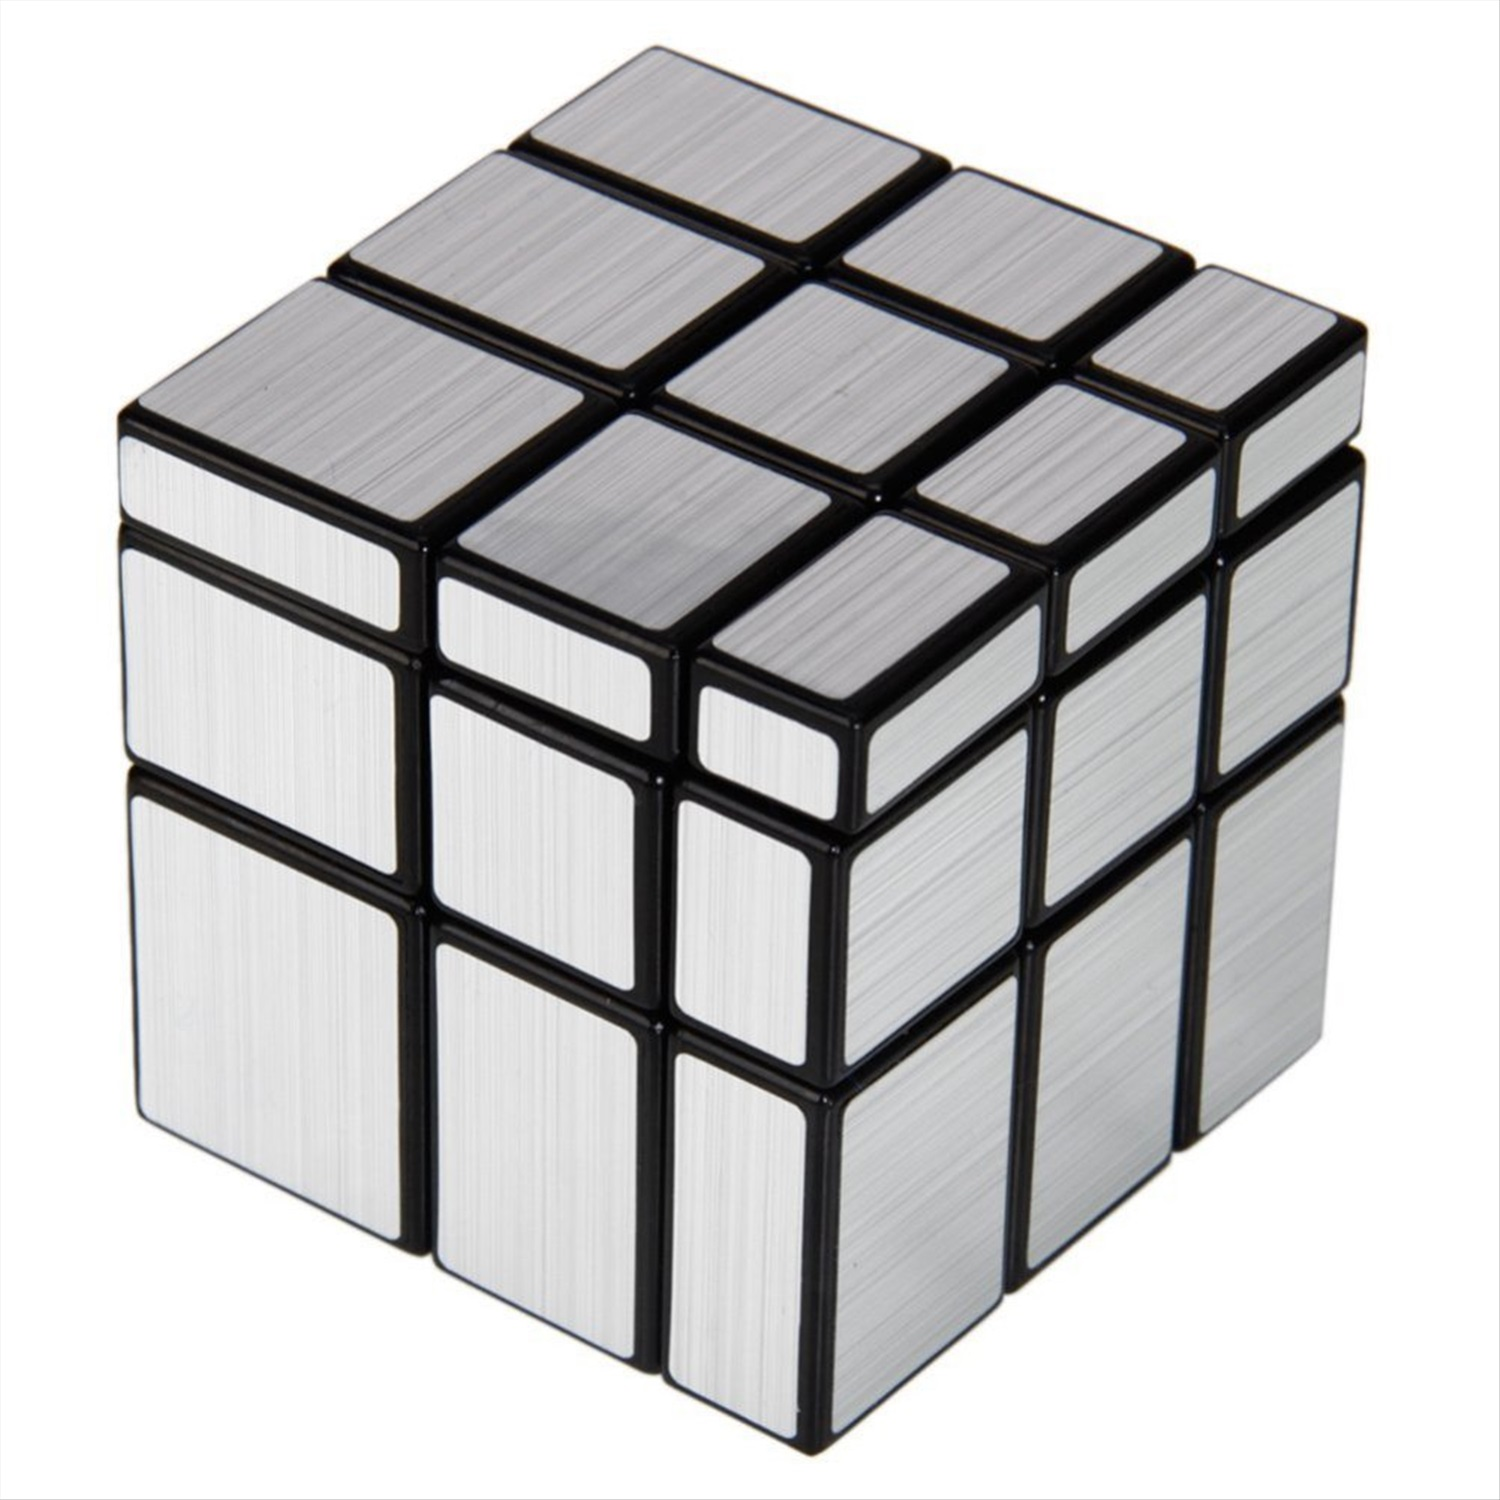
\includegraphics[width=0.3\textwidth]{images/rubic.jpg}
	\\
	Т.е. по каждой координате есть разбиение промежутка бруса на подпромежутки, и для любого набора из подпромежутков по одному для каждой координаты, ему соответсвует брус разбиения. Тогда утверждение про объёмы просто эквивалентно такой формуле:
	\[
		\prod_{j = 1}^n (a_{j,1} + a_{j,2} +\dots+a_{j,m_j}) = \sum_{i_1\in[1,m_1]\dots,i_n\in[1,m_n]} a_{1,i_1}a_{2,i_2}\dots a_{n, i_n}
	\]
	Здесь слева - объём всего большого бруса, а справа сумма объёмов всех маленьких. Сама же формула получается, если просто раскрыть скобки. \\
	
	Чтобы доказать факт для произвольно разбиения бруса, остаётся сказать, что его можно доразбить до такого <<кубик-рубика-подобного>>, 	если продлить все разрезы. Тогда маленькие брусья ещё раздробятся, но мы уже будем знать, что они развны объёму своих частей, при этом сумма всех этих новых маленьких частей будет равна большому брусу, что и даст нам искомое равенство.
\end{anote}

\begin{lemma}
	Объединение, пересечение, разность и симметрическая разность двух элементарных множеств является элементарным множеством.
\end{lemma}

\begin{center}
\begin{tikzpicture}
	\draw[draw=black] (0, 0) rectangle (4, 3);
	\draw[draw=black] (2, 2) rectangle (6, 5);
\end{tikzpicture}
\end{center}

\begin{proof}
	Будем обозначать за $P, Q$ - брусья, а $M, N$ - элементарные множества. Тогда
	\begin{enumerate}
		\item Пересечение. Для начала заметим, что $P \cap Q$ - брус. Значит, $M \cap Q$ - тоже элементарное множество. Ну и отсюда становится очевидным, что $M \cap N$ - элементарное множество.
		
		\item Разность. Для начала, $P \bs Q = P \cap Q^C$, где $Q^C$ - дополнение к $Q$. При этом
		\[
			Q^C = \bigsqcup\limits_{j = 1}^m Q_j
		\]
		где $Q_j$ могут иметь бесконечные рёбра. Допуская такое свойство, получаем, что $P \bs Q$ - брус. Отсюда следующее:
		\[
			M \bs Q = \bigsqcup\limits_{i = 1}^m (P_i \bs Q) \Ra \text{элементарное множество}
		\]
		Ну и тогда
		\[
			M \bs N = M \bs \bigcup\limits_{j = 1}^k Q_j = M \cap \left(\bigcap\limits_{j = 1}^k Q_j^C\right) = \bigcap\limits_{j = 1}^k (M \cap Q_j^C) \text{-конечное пересечение элементарных}
		\]
		
		\item Объединение. 
		\[
			M \cup N = (M \bs N) \sqcup (N \bs M)\sqcup(M\cap N)
		\]
		По доказанном выше, это дизъюнктное объединение трёх элементарных, значит тоже элементарное.
		
		\item Симметрическая разность
		\[
			M \tr N = (M \bs N) \sqcup (N \bs M)
		\]
		Аналогично воспользовались предыдущим результатом.
	\end{enumerate}
\end{proof}

\begin{note}
	Доказанная лемма означает, что совокупность элементарных множеств является \textit{кольцом множеств}. (т.е. кольцо относительно операций $A\tr B$ (<<сложение>>), $A\cap B$ (<<умножение>>)). В качестве нуля - $\emptyset$. (Вообще говоря определение кольца не требует единицы, но если мы ограничимся лишь множествами из единичного куба с центром в начале координат, то её нам удастся получить.)  Теперь в качестве единицы будем дальше брать $K_I$:
	\[
		K_I = \left[-\frac{1}{2}; \frac{1}{2}\right]^n
	\]
	Отметим, что совокупность элементарных подмножеств $K_I$ образует \textit{алгебру множеств}. (Вообще говоря это алгебра над полем $F_2$, но Лукашов отметил, алгебра множеств, это просто кольцо множеств с единицей и нам не стоит связывать это понятие с алгеброй над полем).
\end{note}

\begin{anote}
	Доказать элементарность $P \bs Q \subset \R^n$ можно и другим способом: начнём с того, что разность $P \bs Q$ по одной координате делит промежуток $P$ либо на 1, либо на 2, либо на 3 части. Несложно заметить, что дизъюнктное объединение всех брусьев, образованных при помощи данных подпромежутков (но без такого, что получилось 3 промежутка и мы взяли 2 соседних для какой-то стороны бруса), в точности равно $P$. Осталось понять, что есть только 1 потенциальный брус, который нужно убрать для $P \bs Q$ - это брус, образованный только теми подпромежутками, которые являются подпромежутками $Q$.
	
	Комбинаторно это также означает, что для выражения разности $P \bs Q$ нам всегда достаточно $3^n - 1$ брусьев.
\end{anote}

\begin{theorem} (Свойства объёма на кольце элементарных множеств)
	\begin{enumerate}
		
		\item Если $M, N$ - элементарные множества, то
		\[
			|M \cup N| + |M \cap N| = |M| + |N|
		\]
		
		\item Если $M \subset N$, то $|M| \le |N|$
		
		\item Имеет место конечная аддитивность. То есть
		\[
			M = \bigsqcup\limits_{i = 1}^m M_i \Longrightarrow |M| = \suml_{i = 1}^m |M_i|
		\]
	\end{enumerate}
\end{theorem}

\begin{proof}~
	\begin{enumerate}

		\item[3.] Так как $\forall i \neq j \Ra M_i \cap M_j = \emptyset$ и при этом любое $M_i$ является элементарным множеством, то для $M$ можно записать следующее разбиение на брусья:
		\begin{align*}
			&{\forall i\ \ M_i = \bscupl_{j = 1}^{d_i} P_j^i}
			\\
			&{M = \bscupl_{i = 1}^m M_i = \bscupl_{i = 1}^m \bscupl_{j = 1}^{d_i} P_j^i}
		\end{align*}
		Отсюда получаем следующее:
		\[
			|M| = \sum_{i = 1}^m \sum_{j = 1}^{d_i} |P_j^i| = \sum_{i = 1}^m |M_i|
		\]
		
		\item Просто напишем следующий факт:
		\[
			M \cup N = (M \cap N) \sqcup (M \bs N) \sqcup (N \bs M)
		\]
		Следовательно
		\[
			|M \cup N| + |M \cap N| = 2|M \cap N| + |M \bs N| + |N \bs M| = |M| + |N|
		\]
		Последний переход верен в силу равенства $M = (M \bs N) \sqcup (M \cap N)$ и такого же для $N$.
		
		\item Так как $M \subset N$, то $|N|$ записывается следующим образом:
		\[
			|N| = |M| + |N \bs M| \ge |M|
		\]
	\end{enumerate}
\end{proof}

\begin{definition}
	\textit{$\eps$-расширением($\eps$-растяжением) бруса} $P = \prodl_{k = 1}^n \trbr{a_k; b_k}$ называется брус $P^\eps$:
	\[
		P^\eps = \prodl_{k = 1}^n \left(\frac{a_k + b_k}{2} - \frac{b_k - a_k}{2} \cdot \sqrt[n]{1 + \eps}; \frac{a_k + b_k}{2} + \frac{b_k - a_k}{2} \cdot \sqrt[n]{1 + \eps}\right)
	\]
	Дополнительно отметим, что
	\[
		|P^\eps| = \prodl_{k = 1}^n \big((b_k - a_k)\sqrt[n]{1 + \eps}\big) = |P|(1 + \eps)
	\]
\end{definition}

\begin{definition}
	\textit{$\eps$-сжатием невырожденного бруса} $P = \prodl_{k = 1}^n \trbr{a_k; b_k}$ называется брус $P^{-\eps}$:
	\[
		P^{-\eps} = \prodl_{k = 1}^n \left[\frac{a_k + b_k}{2} - \frac{b_k - a_k}{2} \cdot \sqrt[n]{1 - \eps}; \frac{a_k + b_k}{2} + \frac{b_k - a_k}{2} \cdot \sqrt[n]{1 - \eps}\right]
	\]
	Дополнительно отметим, что
	\[
		|P^{-\eps}| = |P| \cdot (1 - \eps)
	\]
\end{definition}

\begin{note}
	Для любого достаточно малого $\eps > 0$ верно, что $P^{-\eps} \subset P \subset P^\eps$
\end{note}

\begin{theorem} (Счётная(или полная), или $\sigma$-аддитивность объёма на кольце элементарных множеств)
	Если элементарное множество $M$ представлено дизъюнктным объединением счётного числа элементарных множеств $M_i$, то
	\[
		|M| = \row{n = 1}{|M_i|}
	\]
\end{theorem}

\begin{proof}
	Докажем равенство через неравенства в 2 стороны:
	\begin{enumerate}
		\item $\le$. Пусть $M \subset \bscupl_{i = 1}^\infty M_i$. Если сумма объёмов бесконечна, то включение очевидно. Иначе
		\[
			M_i = \bscupl_j P_{ij} \Ra \bscupl_{i = 1}^\infty M_i = \bscupl_{k = 1}^\infty P_k
		\]
		При этом $M = \bscupl_{i = 1}^m Q_i$. Рассмотрим $\eps$-сжатие для каждого невырожденного $Q_i$ (остальные вообще неважны) и $\alpha_k$-растяжения для $P_k$. Тогда
		\[
			\bscupl_{i = 1}^m Q_i^{-\eps} \subset M \subset \bcupl_{k = 1}^\infty P_k^{\alpha_k}
		\]
		Идея состоит в том, что слева стоит замкнутое ограниченное множество, то есть компактное. Значит, из его компактности (так как $P_k^{\alpha_k}$ образуют открытое покрытие):
		\[
			\exists \{k_1, \ldots, k_N\} \such \bscupl_{i = 1}^m Q_i^{-\eps} \subset \bcupl_{l = 1}^N P_{k_l}^{\alpha_{k_l}}
		\]
		Дополнительно $|\bigsqcup_{i = 1}^m Q_i^{-\eps}| = |M|(1 - \eps)$, а в правой части
		\[
			\left|\bigcup_{l = 1}^N P_{k_l}^{\alpha_{k_l}}\right| \le \sum_{l = 1}^N |P_{k_l}|(1 + \alpha_{k_l}) = \suml_{l = 1}^N |P_{k_l}| + \suml_{l = 1}^N \alpha_{k_l} \cdot |P_{k_l}|
		\]
		Если мы положим $\alpha_k := \eps / (|P_k| \cdot 2^k)$ (при $|P_k| = 0$, просто не делим на него), то тогда будет следующая оценка:
		\[
			\left|\bigcup_{l = 1}^N P_{k_l}^{\alpha_{k_l}}\right| \le \row{n = 1}{|P_k|} + \eps \suml_{l=1}^N \frac{1}{2^{k_l}} \le \row{n = 1}{|P_k|} + \eps = \suml_{i = 1}^\infty |M_i| + \eps
		\]
		Полученное неравенство верно для всех достаточно малых $\eps$. Ну и в итоге это даст следующее заключение:
		\[
			(\exists \eps_0 > 0) : (\forall \eps < \eps_0) \emb \left|\bscupl_{i = 1}^m Q_i^{-\eps}\right| = |M|(1 - \eps) \le \left|\bigcup_{l = 1}^N P_{k_l}^{\alpha_{k_l}}\right| \le \sum_{n = 1}^\infty |M_i| + \eps
		\]
		Устремив $\eps$ к нулю, получим нужное неравенство.
		
		\item $\ge$. Теперь $M \supset \bigsqcup_{i = 1}^\infty M_i$. Более того
		\[
			(\forall N \in \N) \emb M \supset \bigsqcup_{i = 1}^N M_i \Ra |M| \ge \suml_{i = 1}^N |M_i|
		\]
		Устремляя $N \to \infty$, получим требуемое.
	\end{enumerate}
\end{proof}